
%%%%%%%%%%%%%%%%%%%%%%%%%%%%%%%%%%%%%%%%%%%%%%%%%%%%%%%%%%%%%%%%%%%%%%%%%%%%%%%%%%
%%% Crawl Gait
%%% 
%%%
%%%%%%%%%%%%%%%%%%%%%%%%%%%%%%%%%%%%%%%%%%%%%%%%%%%%%%%%%%%%%%%%%%%%%%%%%%%%%%%%%%
\chapter{Humanoid Crawl Gait} \label{ch:crawl_gait}

Using the Nao platform, crawling gaits applicable to humanoid robots was explored. 
Not only is crawling a more stable gaiting strategy than walking, but it gives the robot access to areas
of the environment that are inaccessible via walking alone. A low-profile laterally symmetric crawl gait is described, 
modeling the robot as a closed-chain manipulator with pseudo-static dynamics. This gait was parameterized on 
three joint variables and optimized using a cubic splines approach via a genetic algorithm.

As was described in Chapter \ref{ch:navigation}, the gaiting modality directly affects the navigation strategy.
By selecting the appropriate gaiting strategy, the robot can modify its movement to achieve a commanded goal.
This modified movement also modifies which environmental objects present as obstacles.
Expanding the library of gaits legged robots have access to allows robots to be increasingly more capable
and applicable to a wider range of scenarios.

\section{Humanoid Crawling}

Unlike walking and running which enjoy precise definitions, crawling seems to only have a subjective notion.
\cite{Dudek2000} asserts that crawling is a statically stable walk. This definition is problematic
as bipedal gaits have been demonstrated in \cite{figureoutacitation} that are statically stable but would not
be classified as crawling. In addition to this, soldiers performing the high army crawl \cite{armyfieldmanual2008} can be seen to
perform this motion very quickly which introduces a dynamic component to the crawl.
The standard or baby crawl is described as using one's hands and knees to produce forward motion.
In contrast to this, crawls such as the leopard, tiger, bear, and crab use hands and feet to produce
forward motion and the low army crawl uses the hands to drag and one leg to push the body across the ground.
Such diversity in crawling motion makes it difficult to differentiate a crawl from a statically stable
quadrupedal gait that uses something other than the end effectors to interact with the environment.
Despite this, the presented gait produces a motion that many would associate with humanoid crawling.

\subsection{Nao Crawling Limitations}

A primary limitation to the gaits that can be produced by the Nao is the limited number of degrees of freedom (DoF) of the platform
in contrast to the large number of DoF present in humans. While the Nao has 25 DoF, the human body has 244 \cite{zatsiorskybiomechanics}.
The human arm and leg each have 7 DoF while the Nao's arms and legs each have 5. 
Nao's hips have one more degree of freedom, called Hip Yaw-Pitch, which turn the legs together at an angle. 
Figure \ref{fig:nao_hips_legs1} illustrates this degree of freedom more clearly. 
The rest of the DoF of the Nao are in the hands and neck. 
Notably, Nao has no back joint. This prevents the gait designer from prescribing a twisting motion for use in the crawl gait.
These limits in motion preclude the execution of any gaits that require lateral twisting or sagittal arching.
Examples of this are shown in Figure \ref{fig:crawl_back1} .

\begin{figure}
	\vspace*{-0.07in}
	\centerline{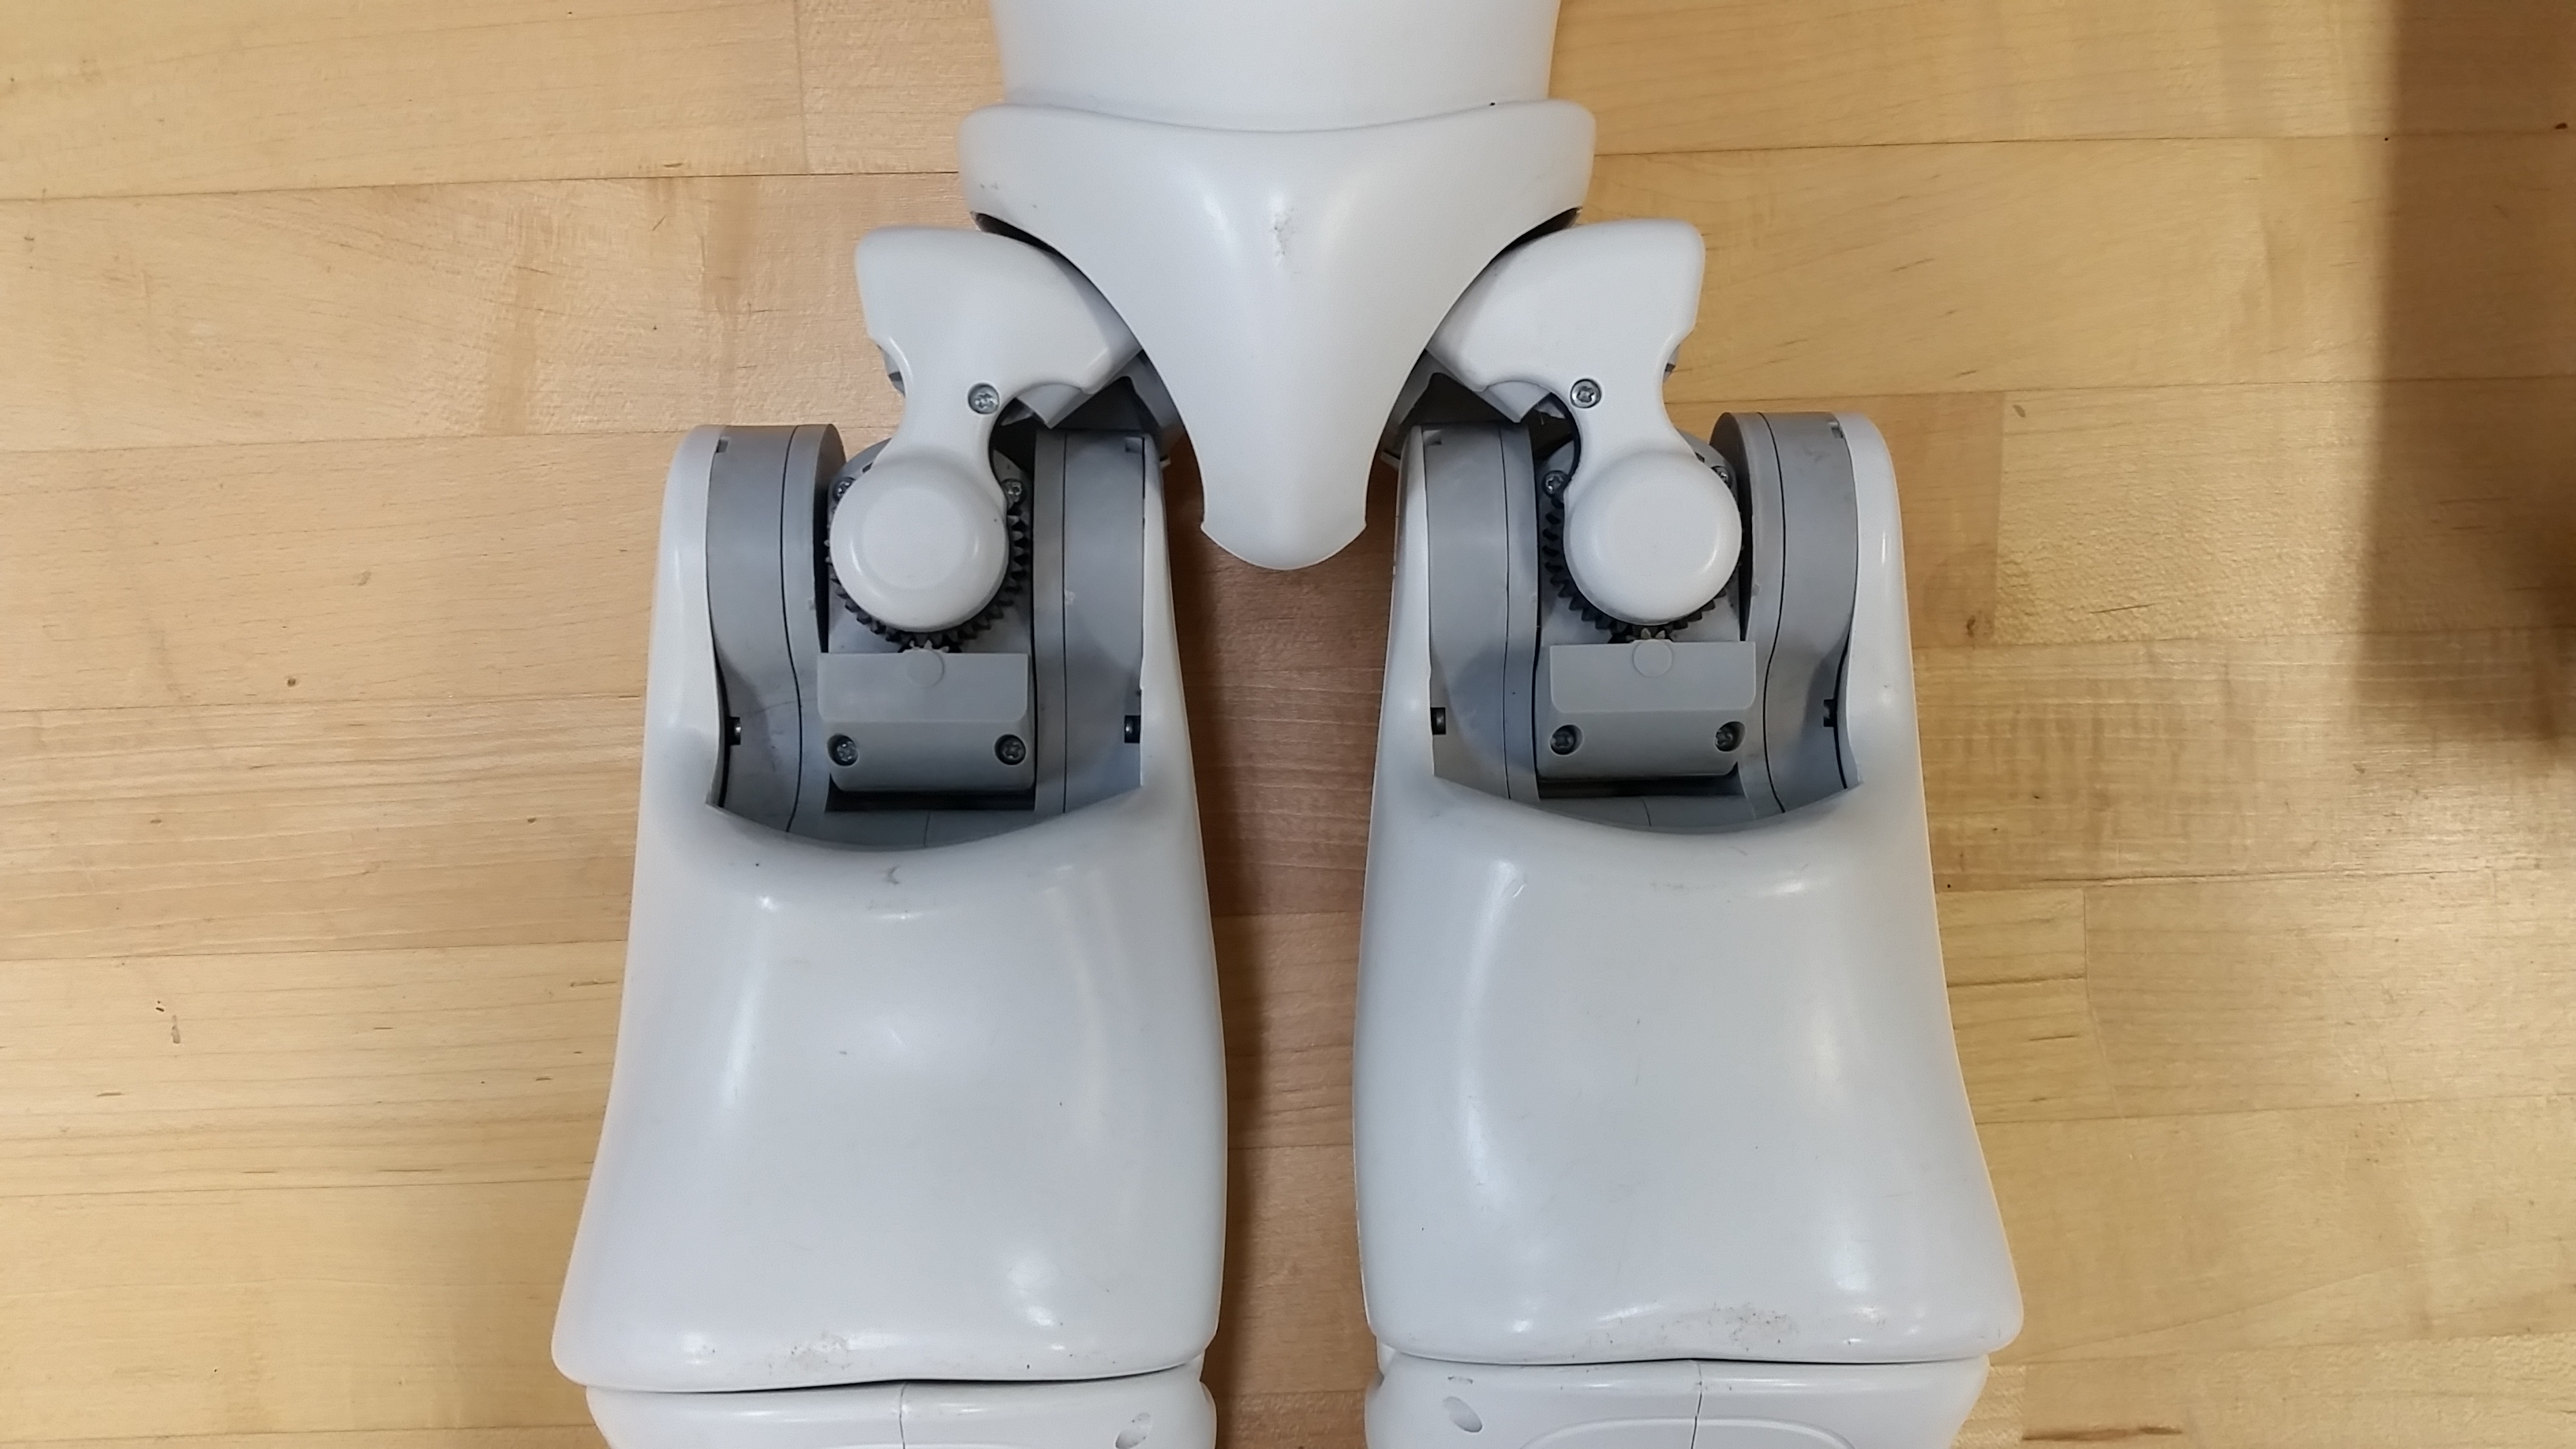
\includegraphics[width=0.395\textwidth]{nao_legs_together1.png}
				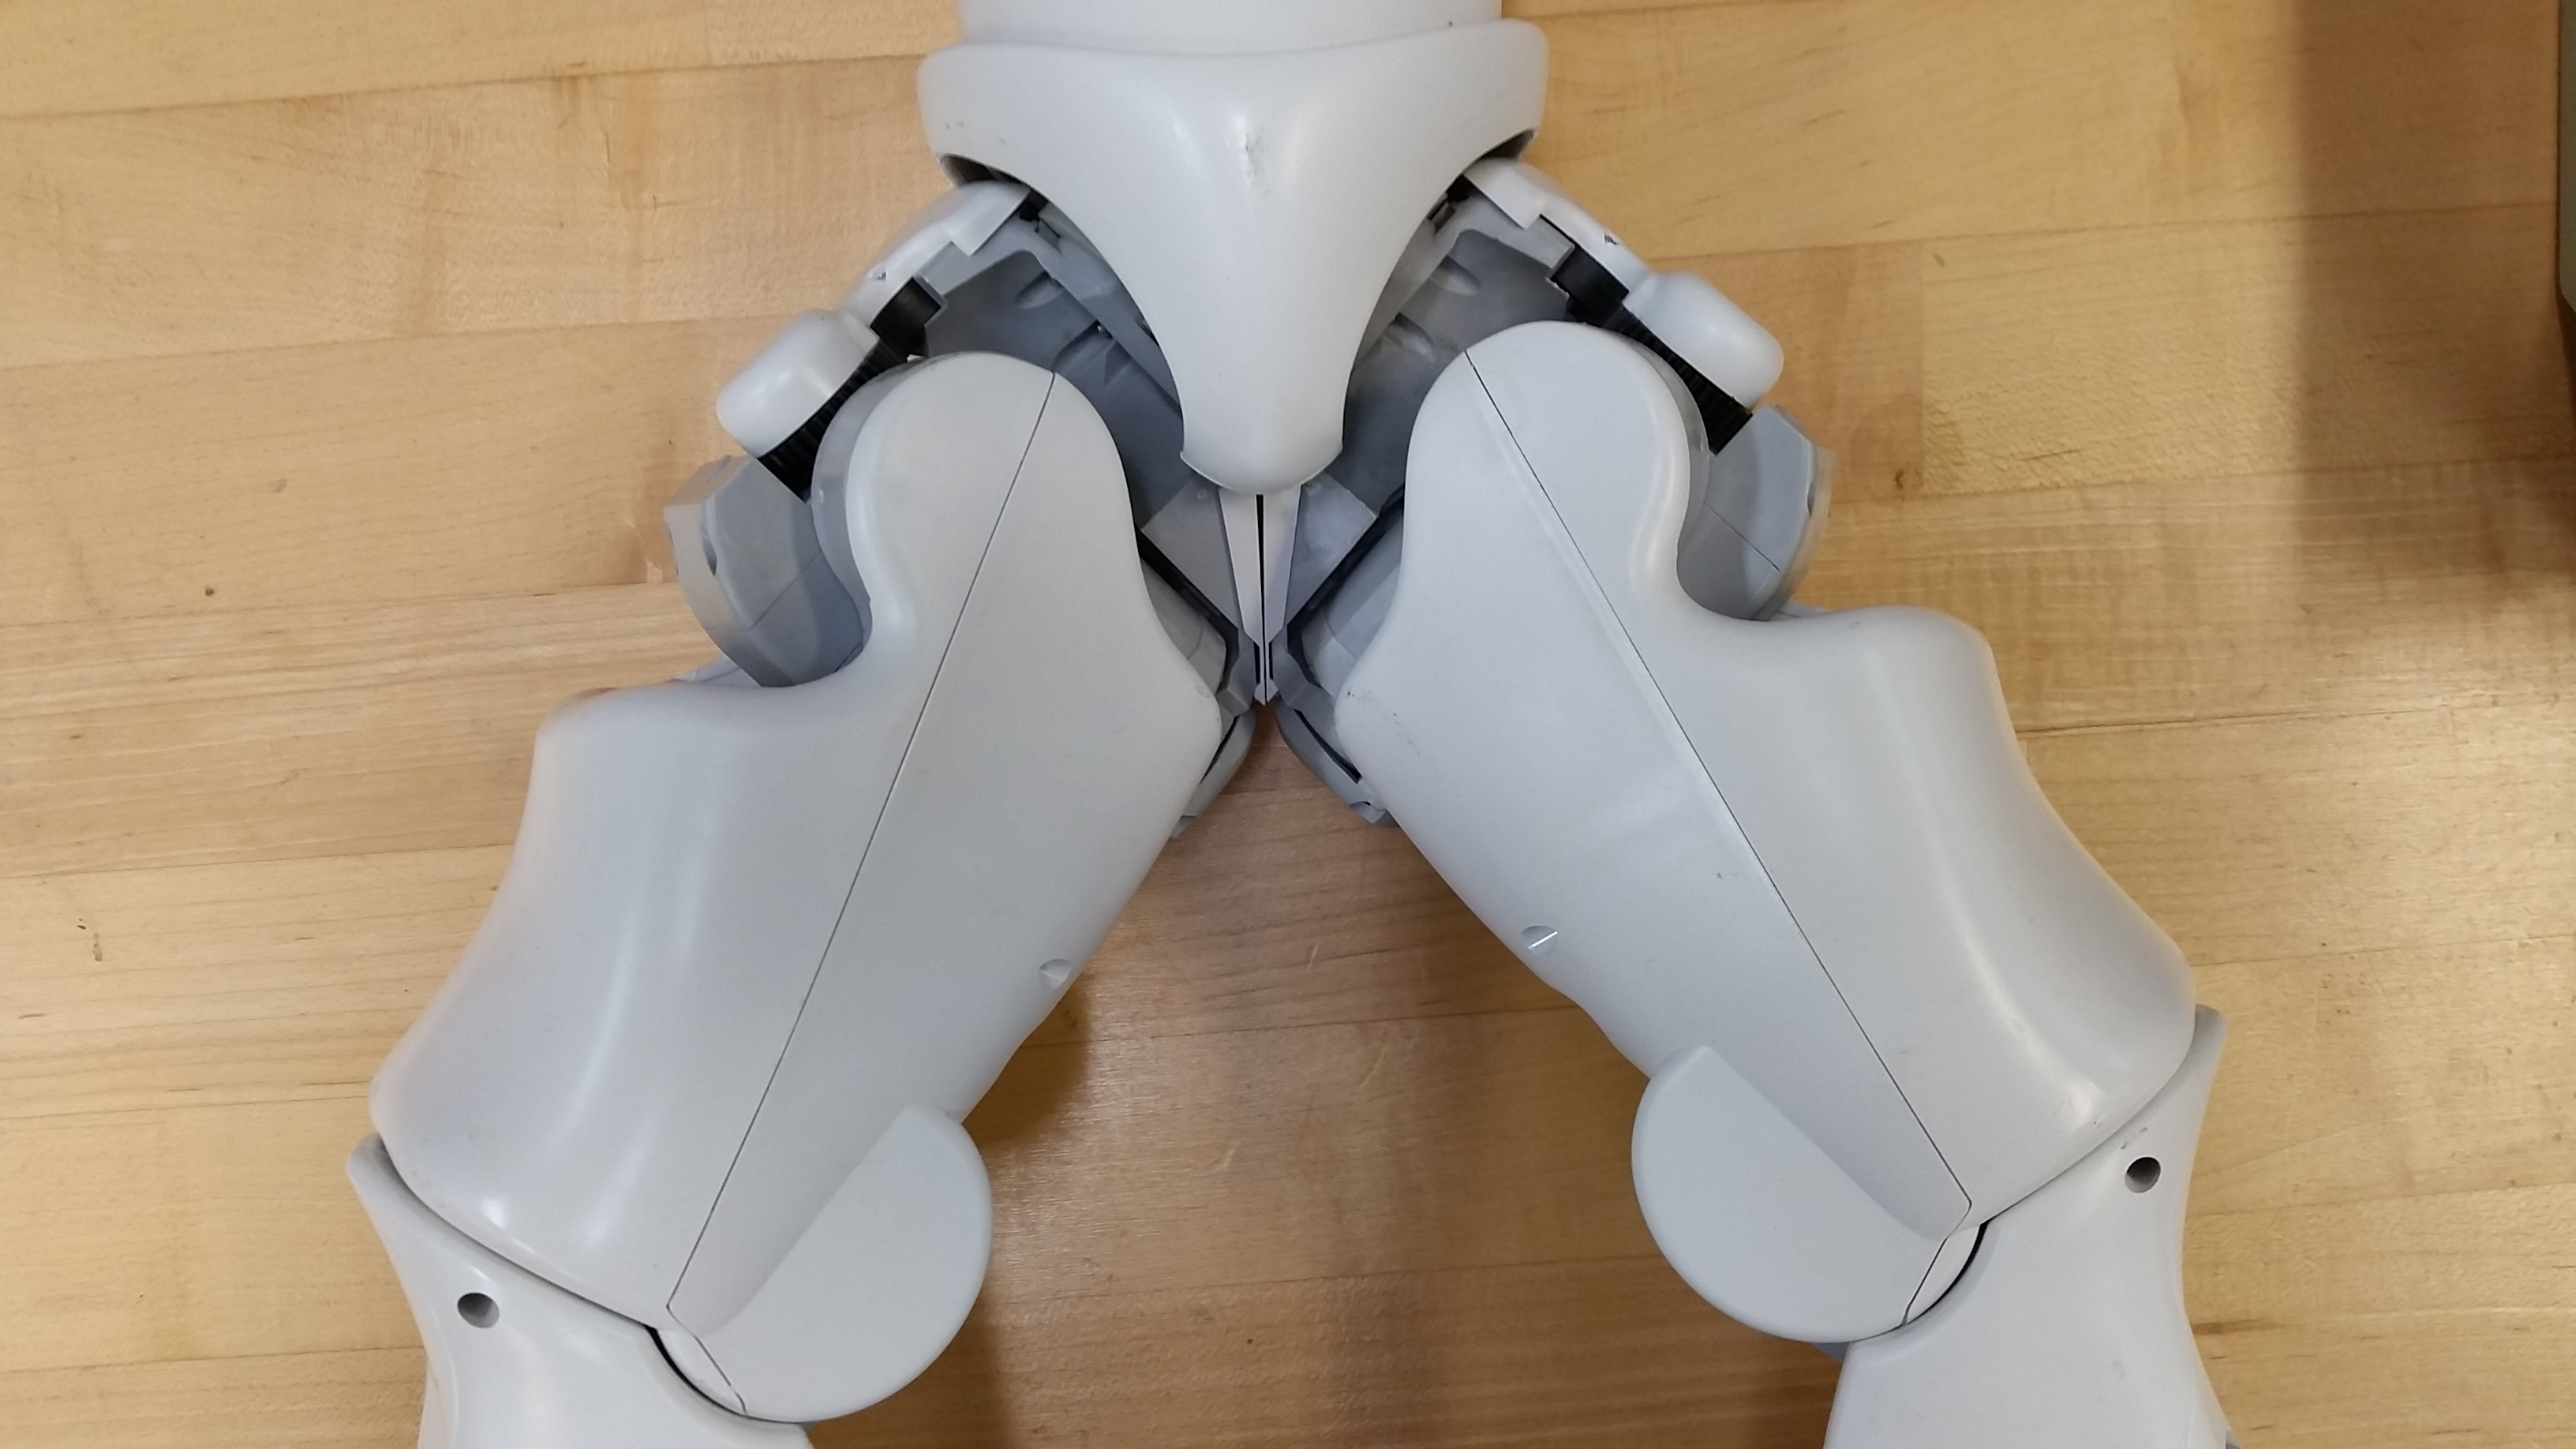
\includegraphics[width=0.5\textwidth]{nao_legs_spread1.png}
				}
	\caption{The pane on the left shows the leg configuration of the Nao when the Hip Yaw-Pitch DoF is fully turned in.
				The right pane show the leg configuration when the Hip Yaw-Pitch is fully turned out. 
				The legs are mechanically linked, making the amount of Hip Yaw-Pitch equal for each leg.}
	\label{fig:nao_hips_legs1}
	\vspace*{-0.2in}
\end{figure}

\begin{figure}
	\centering
	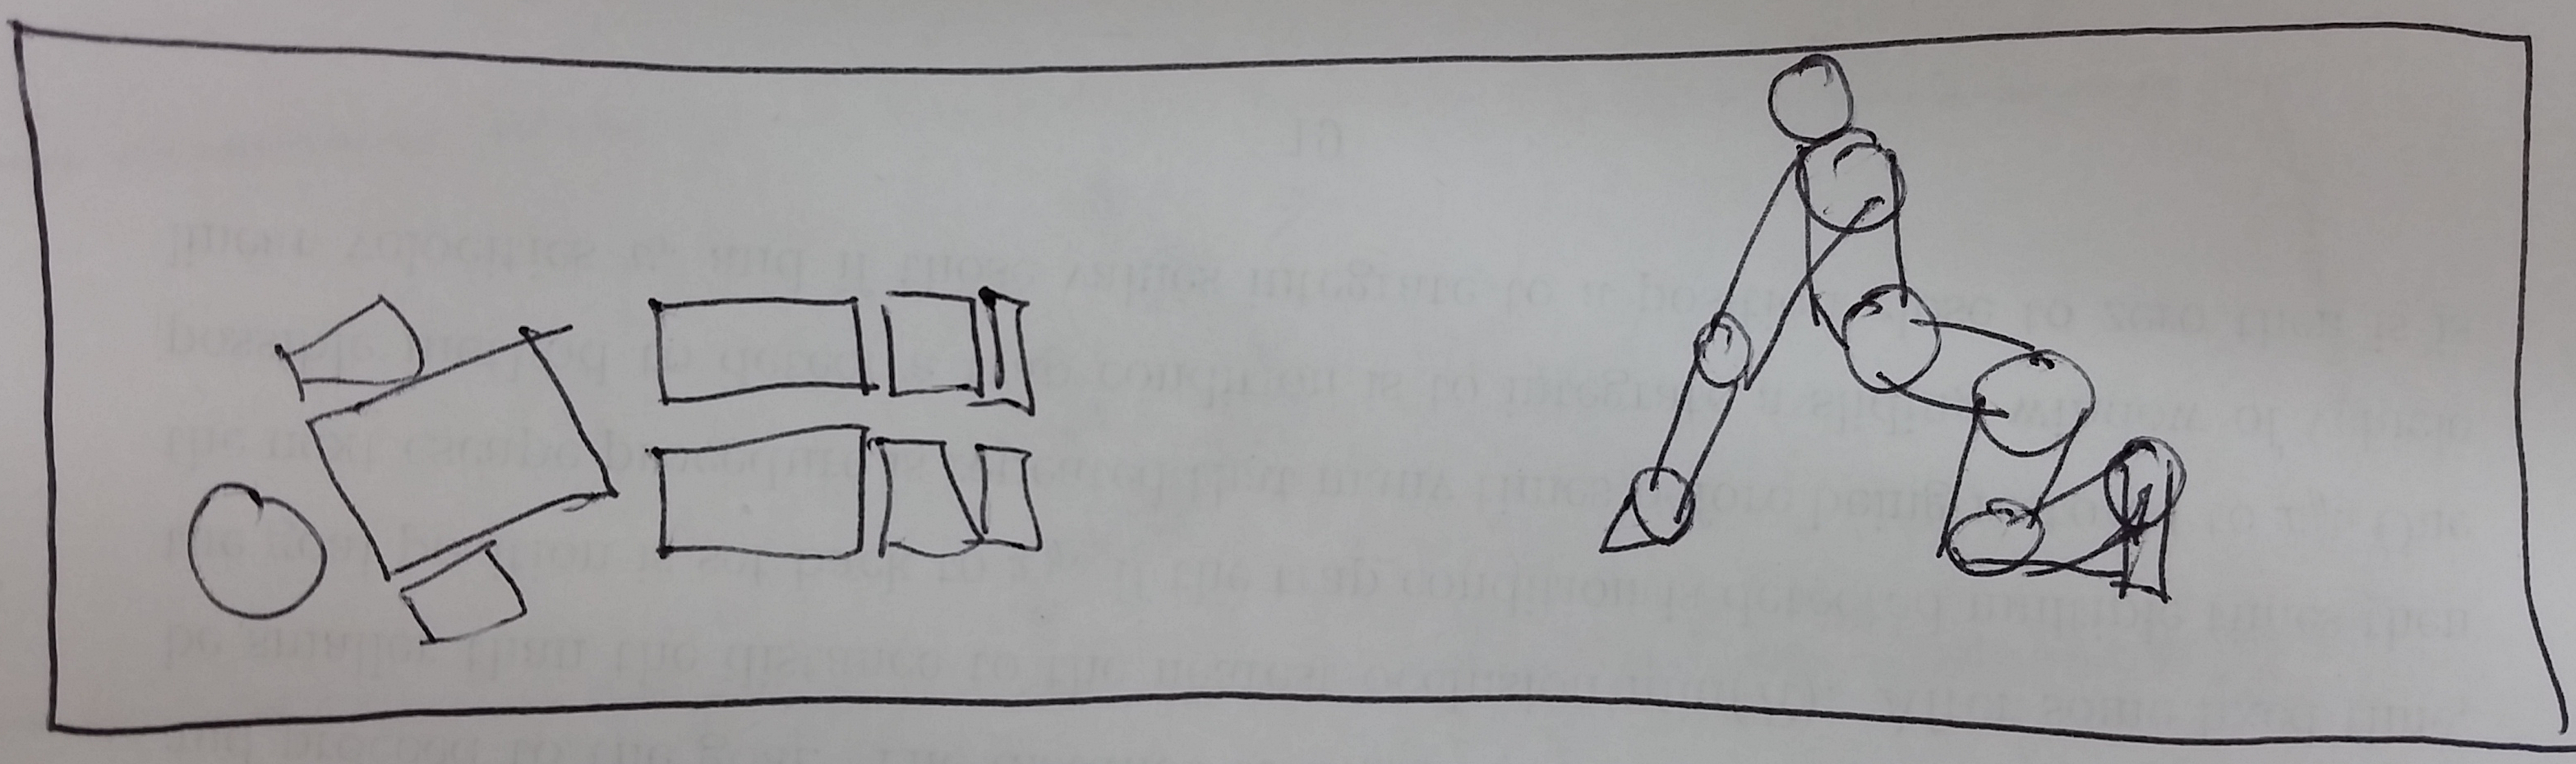
\includegraphics[width=\textwidth]{crawl_back_rough1.png}
	\caption
	{Illustration of crawl motions that involve actuated back joints. The left pane shows lateral twisting during a crawl.
		The right panes shows sagittal arching while on hands and knees.}
	\label{fig:crawl_back1}
\end{figure}

\section{Projected Profile Humanoid Crawl Gait}

The crawling gait presented in this thesis is based on viewing the humanoid form as a set of manipulators on the
sagittal plane. Figure \ref{fig:nao_sideview1} illustrates this concept.
When the robot is laying in the prone position, it necessarily makes contact with the ground. If we then view the robot
from the side (looking at the sagittal plane) we can model it as a planar kinematic chain. If the chest and knees
are making contact with the ground, then the arms from the shoulder joint to the hand, and the legs from the knees to the
toes are free to move without affecting the rest of the body. This produces two open chain manipulators. In the case of the Nao, each has two degrees
of freedom in the sagittal pane, allowing the hands and feet to move independently.
\begin{figure}
	\centering
	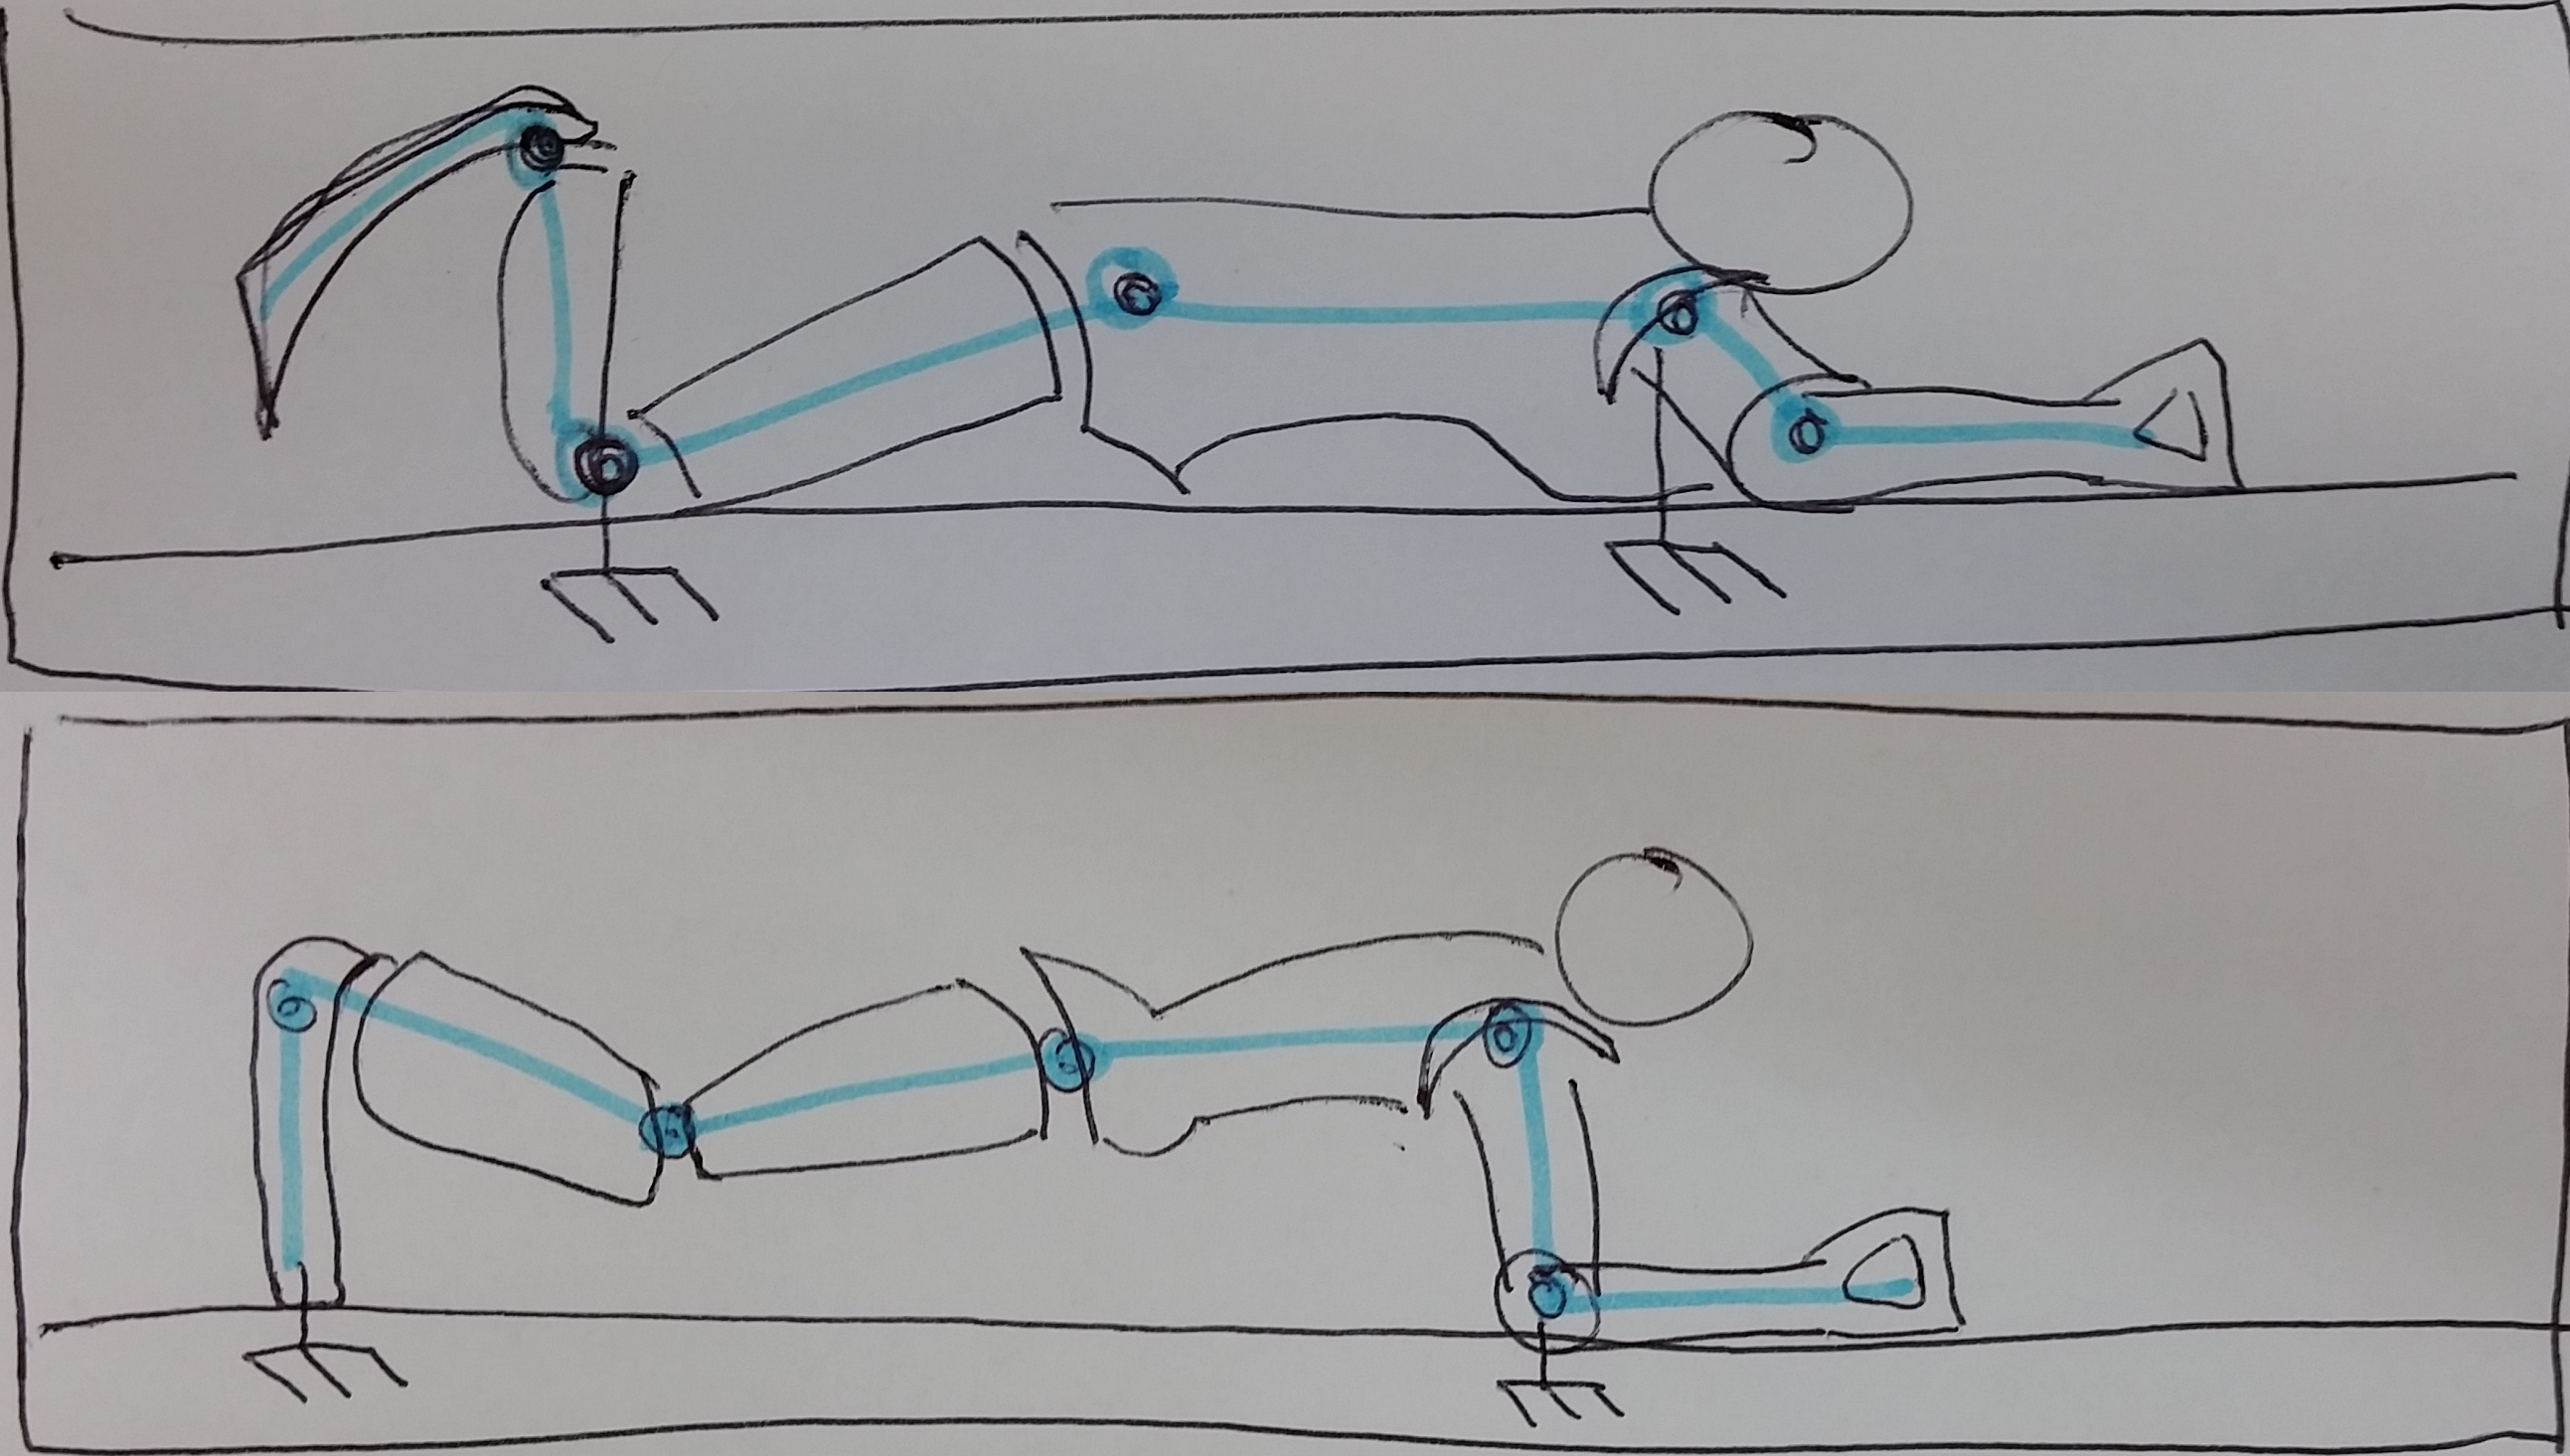
\includegraphics[width=\textwidth]{nao_pp_sagittal_view1.png}
	\caption
	{Illustration of Projected Profile concept. Both panes show the saggital view of the Nao with a schematic representation of the kinematics. 
	In the top view, the robot appears as two open chain manipulators. In the bottom view, the robot appears as one closed chain manipulator.}
	\label{fig:nao_sideview1}
\end{figure}

If the elbows and toes are placed on the ground, then the body from the toes to the elbow can be viewed as a closed chain manipulator.
This allows the joints to work together to move the center of mass. Kinematically, these two phases share two common configurations.
The first configuration is when the elbow is at full extension and the toes touching the knees. We will call this the ``extension" configuration.
This can be viewed as the robot reaching forward. The second is when the elbow is at full flexion and the ankles at extension.
We will call this ``compression".
This can be viewed as the robot having pulled itself forward. These motions can then be combined
to produce a full gait.

Using the Nao robot as an example, Figure \ref{fig:nao_phases1} shows the full gaiting sequence.
The robot initializes itself in the open chain configuration. From this, it can position
its end effectors (the toes and elbows) into the first common configuration ``extension". Next, the robot is in the closed chain 
configuration in which it can transport its center of mass forward until it reaches the ``compression" configuration. Finally the robot
is again in the open chain configuration and the cycle can start again.

\begin{figure}%[!th]
	\centerline{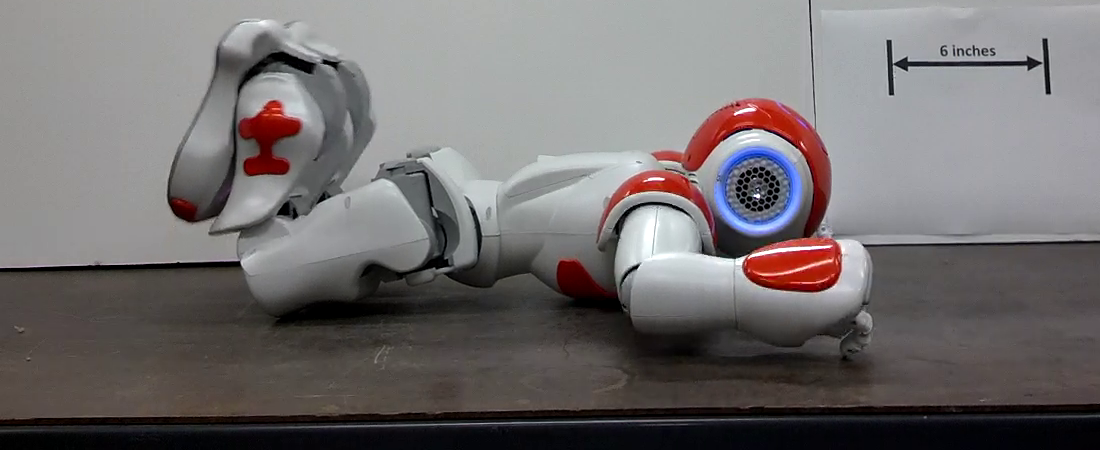
\includegraphics[width=0.5\textwidth]{White_Background/1_onBellyBegin.png}
				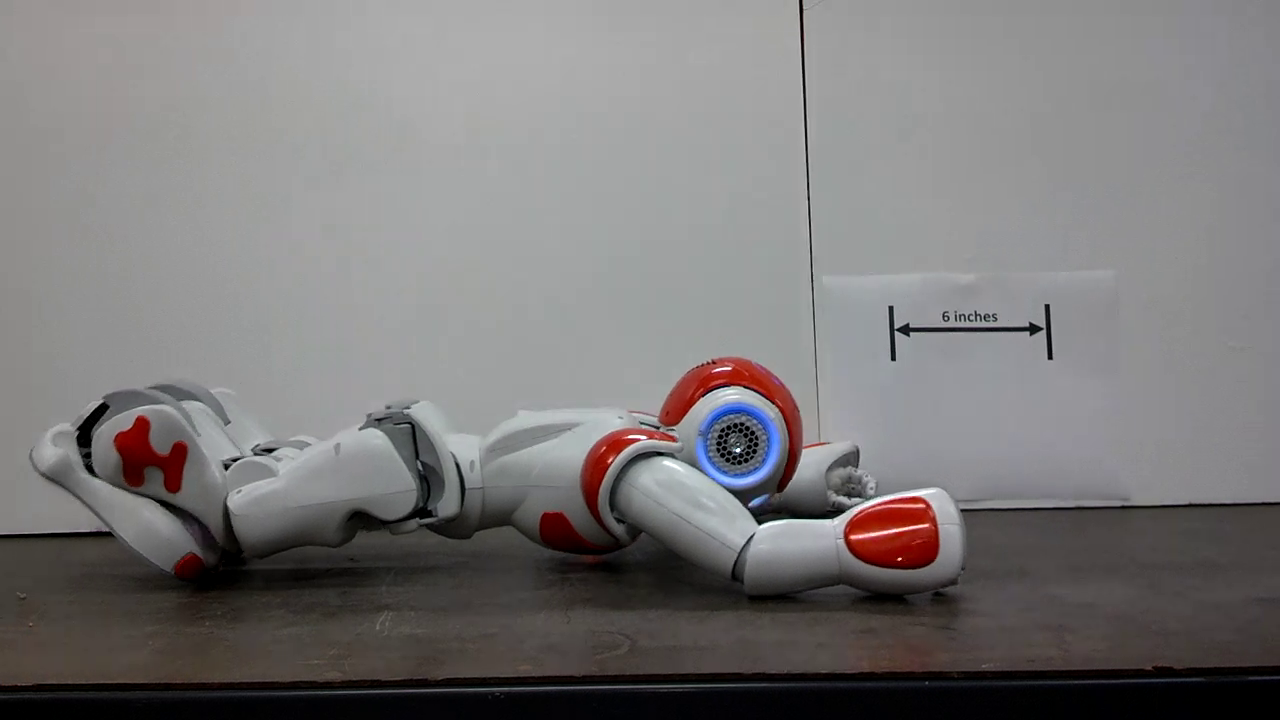
\includegraphics[width=0.5\textwidth]{White_Background/2_extension.png}
				}

	\vspace*{0.05in}

	\centerline{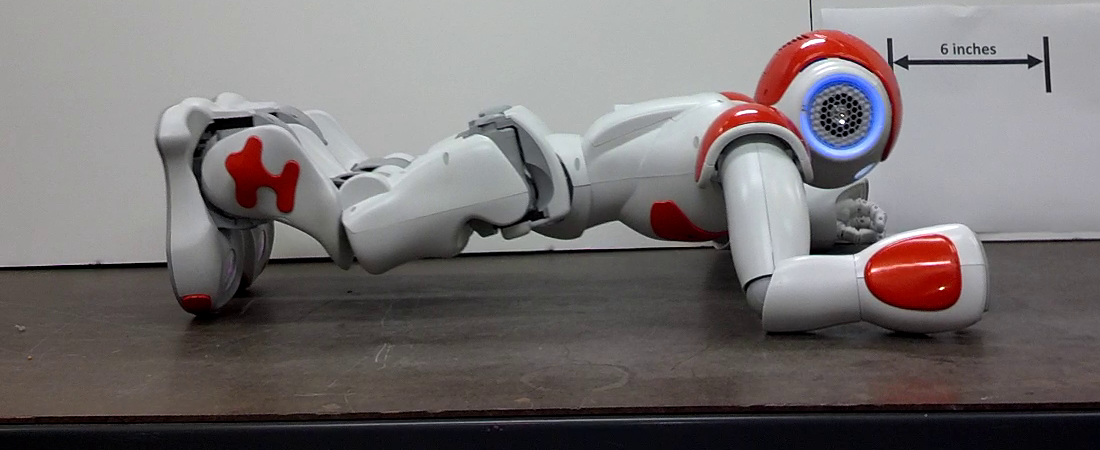
\includegraphics[width=0.5\textwidth]{White_Background/3_apex.png}
				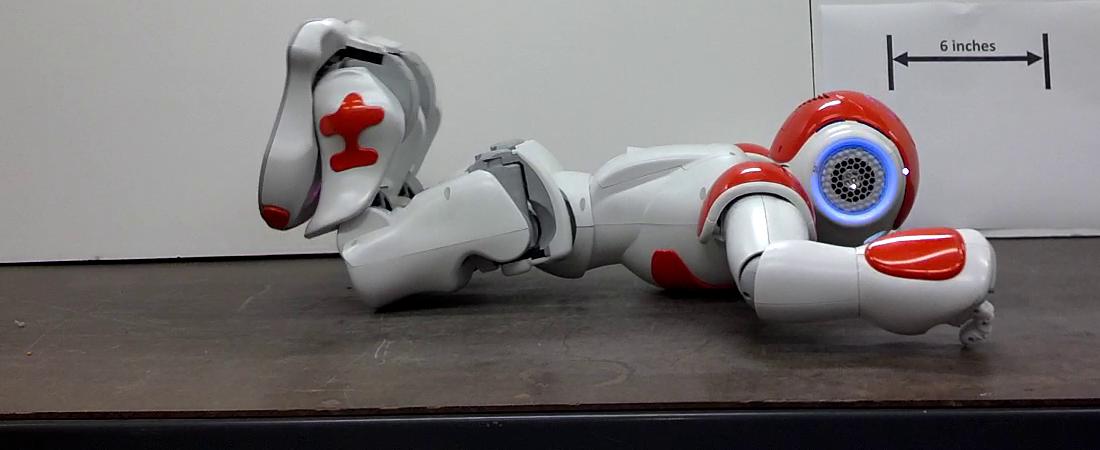
\includegraphics[width=0.5\textwidth]{White_Background/5_onBellyEnd.png}
				}
	\caption{The above sequence shows the motion segments and robot postures in the crawl gait. 
				The upper left pane shows the initial open chain configuration. The upper right
				pane moves the robot to the ``extension" configuration. The lower left
				shows the ``compression" configuration. Finally, the lower right shows the 
				robot, having translated forward, once again in the open chain configuration.
				A 6-inch marker is shown in the background as a length scale reference.}
	\label{fig:nao_phases1}
\end{figure}

The gait is laterally symmetric. 
If we actuate the joints at an appropriate rate, dynamic effects from the robot's motion do not become a significant factor.
As detailed in Chapter \ref{ch:results}, this gait can be performed on the Nao at a speed of 1 ft every 6 to 8 seconds. 
The wide surface area of the forearm provides a high coefficient of friction against slipping and the small surface area of
the toes can act as a point of high pressure which can dig into soft surfaces such as carpets.
The gait is statically stable in the sense that the robot's motion can be paused at any point and the robot will maintain that pose.
The gait does not depend on the robot
sliding along the surface nor does it highly depend on surface friction to pull the robot forward.
The gait has a very low profile. The highest point on the robot during the gait (which is the top of the head)
is about 8 inches off of the ground. In contrast, during walking, the Nao robot stands 23 inches tall.

\subsection{Open Chain Kinematics}
The Projected Profile crawl gait has two kinematic configurations: open chain and closed chain. In the open chain
configuration, the robot acts as two independent planar manipulators. 
Each manipulator has two degrees of freedom as can be seen in Figure \ref{fig:open_chain1} .

\begin{figure}
	\centering
	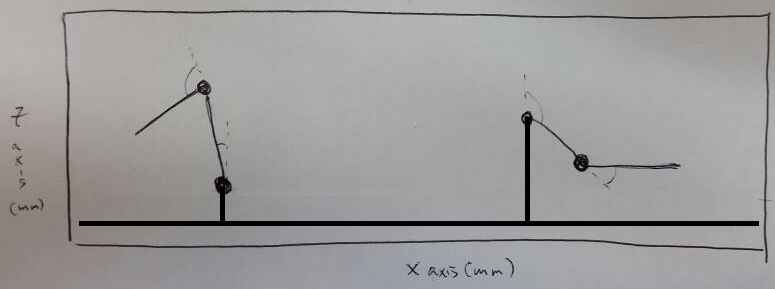
\includegraphics[width=\textwidth]{stick_open_chain_rough1.png}
	\caption
	{Simplified kinematic model of the sagittal projection of the open chain configuration.
	The manipulator on the left represents the tibia-foot chain. The manipulator on the right
	represents the humerus-forearm chain. The origin of the knee and shoulder are represented as 
	having a z-axis offset because the knee and chest of the robot have heights that raise their 
	origins.}
	\label{fig:open_chain1}
\end{figure}

With the Nao facing downwards, the feet towards the origin and the head in the positive x direction, 
the forward kinematics for each manipulator are described by:
\begin{align}
	x &= x_0 + l_1 cos(\theta_1) + l_2 cos(\theta_1 + \theta_2) \\
	z &= z_0 + l_1 sin(\theta_1) + l_2 sin(\theta_1 + \theta_2)
\end{align}
where $x_0$ and $z_0$ are the superior and posterior offsets with respect to the global frame, respectively. $l_1$ is the length of the
humerus/tibia, $l_2$ is the length of the forearm/foot, $\theta_1$ is the angle subtended by the 
shoulder/knee and the x-axis, and $\theta_2$ is the angle subtended by the ankle/elbow and the x-axis of the humerus/tibia.

The solutions to the inverse kinematics problem can be seen as:

\begin{align}
	\theta_2 &= \cos^{-1} \left (\frac{(x - x_0)^2 + (z - z_0)^2 - l_1^2 - l_2^2}{2 l_1 l_2} \right ) \label{eq:open_fk_eq1}\\
	\theta_1 &= 2 \tan^{-1} \left (\frac{-B \pm \sqrt{B^2 - 4AC}}{2A} \right ) \label{eq:open_fk_eq2}\\
	A &= (x - x_0) + (z - z_0) + l_1 + l_2 (\cos(\theta_2) + \sin(\theta_2)) \\
	B &= -2(l_1 + l_2(\cos(\theta_2) - \sin(\theta_2)) \\
	C &= (x - x_0) + (z - z_0) - l_1 - l_2 (\cos(\theta_2) + \sin(\theta_2))
\end{align}

This solution derives from the standard inverse kinematics procedure of inverting the forward kinematics.
$\theta_1$ must be chosen such that no part of the robot tries to intersect with the floor. 
In practice, the two argument arc-tangent function $atan2$ is used instead of $\tan^{-1}$ .

%%% Projected profile %%%
\subsection{Closed Chain Kinematics}

The closed chain configuration models the toes and elbows of the robot as being fixed to the ground.
As with all closed chain kinematics, describing the forward kinematics requires solving an inverse
kinematics equation. Modeling the robot in the same orientation as the open chain, with the toe at the origin
and neglecting the thickness of the elbow,
the forward kinematics of the closed chain are:

\begin{align}
	d_e &= \sum_{i=1}^5 l_i \cos(\sum_{j=1}^i \theta_j) \label{eq:fk_eq1}\\
	0 &= \sum_{i=1}^5 l_i \sin(\sum_{j=1}^i \theta_j) \label{eq:fk_eq2} \\
	\alpha &=\sum_{i=1}^5 \theta_i \label{eq:fk_eq3}
\end{align}
where $d_e$ is the prescribed distance of the elbow from the foot and $\alpha$ is the desired angle
created by the x-axis of the humerus and the ground.
$\theta_1$ through $\theta_5$ are the angles of the following joints with respect to their previous links when projected onto the sagittal plane:
toe-to-ground, ankle, knee, hip, shoulder. In Figure \ref{fig:pp_stick1}, the red lines represent the links projected onto the sagittal plane.
These equations are the standard planar manipulation equations, treating the foot as the base link 
with the elbow as the end effector.
Equation \ref{eq:fk_eq1} constrains the end effector to be a set distance from the foot and 
equation \ref{eq:fk_eq2} constrains the end effector to be on the ground.
Using equation \ref{eq:fk_eq3}, equations \ref{eq:fk_eq1} and \ref{eq:fk_eq2} can be rewritten as:

\begin{align}
\sum_{i=1}^4 l_i \cos(\sum_{j=1}^i \theta_j) &= d_e - l_5 \cos(\alpha) \label{eq:sum_cos1} \\
\sum_{i=1}^4 l_i \sin(\sum_{j=1}^i \theta_j) &= - l_5 \sin(\alpha). \label{eq:sum_sin1}
\end{align}

\begin{figure}
	\centering
	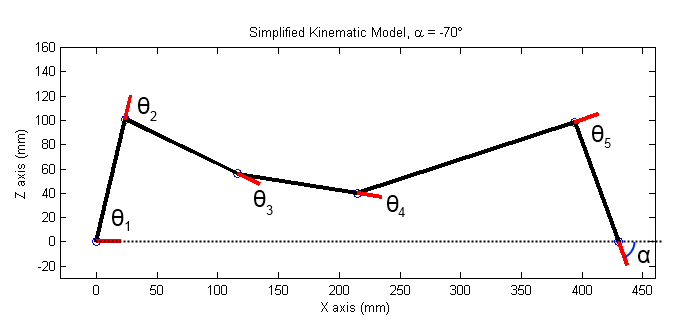
\includegraphics[width=\textwidth]{stick3_with_notation1.png}
	\caption
	{Simplified kinematic model of the sagittal projection of the closed chain configuration.}
	\label{fig:pp_stick1}
\end{figure}

If $\theta_3$, $\theta_4$, and $\alpha$ are prescribed angles, then equations \ref{eq:sum_cos1} and \ref{eq:sum_sin1} are two equations 
in the two unknowns $\theta_1$ and $\theta_2$. 
$\theta_3$ and $\theta_4$ can be constant or time-varying as the resultant configuration is a function of these two ``free" variables.
Taking the square of each of the equations \ref{eq:sum_cos1} and \ref{eq:sum_sin1}, 
an equation in the single variable $\theta_2$ is obtained as:
\begin{align}
	2l_1 K_1 \cos(\theta_2) + 2l_1K_2 \sin(\theta_2) &= [d_e - l_5 \cos(\alpha)]^2 + [l_5 \sin(\alpha)]^2 - l_1^2 - K_1^2 - K_2^2 \label{eq:theta2_eq1} \\
	K_1 &= l_2 + l_3 \cos(\theta_3) + l_4 \cos(\theta_3 + \theta_4) \label{eq:theta2_eq2}\\
	K_2 &= -l_3 \sin(\theta_3) - l_4 \sin(\theta_3 + \theta_4) \label{eq:theta2_eq3}
\end{align}

The solution to equation \ref{eq:theta2_eq1} is of similar form to that seen in \ref{eq:open_fk_eq2}.
In general, there will be two solutions for $\theta_2$, but one of them will cause the robot to collide
with the ground and must be guarded against.
With $\theta_2$ solved, equations \ref{eq:sum_cos1} and \ref{eq:sum_sin1} can be used to solve for $\theta_1$:
\begin{align}
	\theta_1 = tan^{-1} \left( \frac{sin(\theta_1)}{cos(\theta_1)} \right ) \label{eq:theta1_eq1}\\
	cos(\theta_1) = \frac{K_3 (d_e - l_5 \cos(\alpha)) + l_5 K_4 \sin(\alpha)}{K_3^2 + K_4^2} \label{eq:theta1_eq2}\\
	sin(\theta_1) = \frac{K_4 (d_e - l_5 \cos(\alpha)) - l_5 K_3 \sin(\alpha)}{K_3^2 + K_4^2} \label{eq:theta1_eq3}\\
	K_3 = l_1 + K_1 cos(\theta_2) + K_2 sin(\theta_2) \label{eq:theta1_eq4}\\
	K_4 = K_2 cos(\theta_2) - K_1 sin(\theta_2) \label{eq:theta1_eq5}
\end{align}

Lastly, $\theta_5$ is solved using equation \ref{eq:fk_eq3}.

% Robot is like a parallelogram. Any robot that can make a parallelogram can use this principle.
With these angles solved, the entire robot is parameterized on three angles $\theta_3, \theta_4, \alpha$.
If $\theta_3$ and $\theta_4$ are fixed, then starting with the elbow at full extension, bringing the elbow
to flexion moves the robot forward. This corresponds to $\alpha$ starting with a small negative angle and 
ending with a large negative angle. 
For the Nao, $\alpha$ is initialized at approximately $-30^\circ$ and terminates at about $-90^\circ$ .
The primary intuition about this procedure is that the closed chain is like a parallelogram that is used to shift
the mass of the robot. Any robot (humanoid or not) that can be set into this configuration can use this 
framework in order to gait the robot.

\subsection{Application onto Nao}
Once the projected profile time sequence of angles has been computed, it needs to be applied to the Nao.
Figure \ref{fig:nao_pp_view1} illustrates the sagittal view of the robot in the closed chain configuration.
When Nao is set to this configuration, the ankle pitch, knee pitch, hip pitch, and shoulder pitch joints 
of the robot directly correspond to $\theta_2$ through $\theta_5$. $\theta_1$ corresponds to the angle
subtended by the robot's foot and the ground. Unlike the first five joint angles, angle $\alpha$ does not have a
direct correspondence and must be derived from the projection of the arm onto the sagittal plane $n_p$ . 

\begin{figure}
	\includegraphics[width=\textwidth]{horz_profile_with_notation2.png}
  	\caption{Sagittal view the Nao in the closed chain crawling configuration. 
  				The locations of the joints used in the projected profile calculation are shown as blue dots. 
  				$n_p$ represents the sagittal plane of the robot.
  			}
  	\label{fig:nao_pp_view1}
\end{figure}

[More to come on this part. Continue reading.]

%%% Pseudo-static modelling %%%
\section{Optimization}

In the previous section, the Projected Profile crawl gait was parameterized on angle triplet $[ \theta_3, \theta_4, \alpha ]$ .
To achieve a crawling gait, $\theta_3$ and $\theta_4$ can be set to be constant and $\alpha$ linearly incremented
from an initial angle to a final angle as a function of time. While this configuration successfully gaits the robot,
it is heuristic. To improve the approach, the selection of this triplet as a function of time is considered as an optimization 
problem. While many different quantities such as gait speed or the levelness of the back (for transportation of payloads) could
be considered as optimization metrics, in this thesis the energy usage was minimized via joint torque measurements.
The aim was to increase the amount of time the crawling gait could be performed and reduce the stress on the robot's joints.

\subsection{Pseudo-static Model}

In order to optimize the gait with respect to the joint torques of the robot, a dynamic model of the robot is required.
As the Projected Profile crawl gait is conceived as a statically stable gait and performed at slow speeds,
the dynamics due to the movement of the robot are not considered to be forces that the 
motor controllers must counteract. 
During any part of the gait the robot will not slide if the gaiting direction is orthogonal to gravity and
if the robot were to relax its joints it would collapse.
Considering this, the resultant joint torques can be seen to be a function of gravity. 
This pseudo-static model of the robot can then be used to produce cost metric for the optimization procedure.
While conceptually simple, analyzing the projected profile closed chain manipulator to produce the 
system dynamics is challenging.
In lieu of this, the robot was simulated for different values of the angle triplet in the closed chain 
configuration to generate a table of torques. This table of torques is then interpolated to produce
a model of joint torques as a function of the parameterized angles:
\begin{equation}
	[\tau_2, \tau_2, \tau_4, \tau_5] = jointTorques(\theta_3, \theta_4, \alpha)
\end{equation}
where $\tau_2, \tau_3, \tau_4, \tau_5$ are the torques of one of the ankles, knees, hips, and shoulders, respectively.
In this case, only one of each of the joints is considered because the gait is laterally symmetric. This means
the torque of the left joint should be the same of the right joint.
$\tau_1$ is not a product of the function as $\theta_1$ is not an actuated joint.

The V-REP simulator by Coppelia Robotics was used to gather joint torque data. It uses the Open Dynamics Engine (ODE)
as its dynamics solver and is distributed with a model of the Nao Humanoid Platform. The model of the Nao
kinematically corresponds with the Nao V4 and has the same mass values for the links. 
The Nao V4 is the robot used in this thesis.
It has an easy to use API that can interface with C++, Python, or MATLAB.

\begin{figure}
	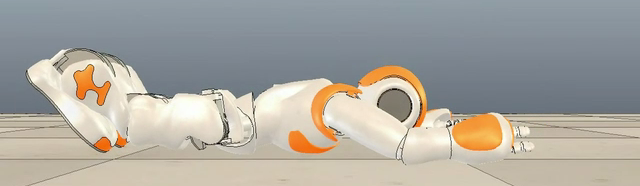
\includegraphics[width=\textwidth]{nao_vrep1.png}
  	\caption{ A sample screen capture of the V-REP simulation of the Nao robot in the closed
  				chain configuration. The robot is set to different poses and then the joint torques
  				are read after a short settle time.
  			}
  	\label{fig:nao_vrep1}
\end{figure}

Figure \ref{fig:nao_vrep1} shows a screen capture of the Nao model in the V-REP simulator. 
The Nao was configured to be in the closed chain and set to different joints angles. 
The initial and final values of $\alpha$ were constrained due to the gaiting requirement of the elbow to start at 
extension and end at flexion. The ranges of $\theta_3$ and $\theta_4$ were defined according to what seemed
like plausible knee and hip angles for the gait. Using these limits a discrete set of triplets were defined
at a $2.5^\circ$ resolution for each triplet parameter. These triplets were sent through the kinematics equations to produce the joint
commands for the simulated Nao robot. 
Table \ref{tab:angle_set_params1} lists the parameters that describe the triplets tested. In total, 9,975
different joint configurations were simulated.
To allow for the effect of
any dynamics generated by the change in configuration to settle, the torque values of each of the joints was recorded
after a period of one second.

\begin{table}
	\centering
	\begin{tabularx}{0.65\textwidth}{|X||X|X|}
		\hline
		\textbf{Configuration Parameter} 	&	\textbf{Minimum Angle (degrees)} 		&	\textbf{Maximum Angle (degrees)} 	\\	\hline\hline
		$\theta_3$ 							& 	-5										&	45	 								\\	\hline
		$\theta_4$							&	15										&	-30									\\ 	\hline
		$\alpha$							&	-30										&	-90									\\ 	\hline
	\end{tabularx} 
	
	\caption{Table of initial and final joint angles for each angle in the configuration triplet used to generate the set of
				angles used to configure the simulated Nao robot.
				The resultant set had 9,975 configurations with an angular resolution of $2.5^\circ$.}
	\label{tab:angle_set_params1}
\end{table}

%%% Optimization procedure %%%
\subsection{Optimize <-------- Everything after this still needs to be edited}

As a requirement of the gait, the initial and final poses for the closed chain phase needed to be common to the
open chain phase of the gait. 

Now that we have things set up and we have our model/function/table thing we can try to optimize the gait.
The method of optimization we used was a genetic algorithm on cubic splines. We knew where the parameters have to start
and end so we set the cubics terminations there. We told it to do it in 1 second because we knew that would work
as the crawl with the constants works.
Optimization cost was this: ... which we weighted according to which joints were stronger.
We threw this into a basic genetic algorithm which tweaked the 12 parameters (4 for each configuration spline)
and iterated on this X many times. 

New.


